\documentclass{whiteboard}
\begin{document}
\begin{frame}[plain,t]
\bbcover{OJ 10369}{Arctic Network}{Prof. Edson Alves}{Faculdade UnB Gama}

\end{frame}
\begin{frame}[plain,t]
\vspace*{\fill}

\bbenglish{The Department of National Defence (DND) wishes to connect several northern outposts by a wireless network.  Two different communication technologies are to be used in establishing the network: every outpost will have a radio transceiver and some outposts will in addition have a satellite channel.}

\vspace{0.1in}

\bbenglish{Any two outposts with a satellite channel can communicate via the satellite, regardless of their location. Otherwise, two outposts can communicate by radio only if the distance between them does not exceed $D$, which depends of the power of the transceivers. Higher power yields higher $D$ but costs more. Due to purchasing and maintenance considerations, the transceivers at the outposts must be identical; that is, the value of $D$ is the same for every pair of outposts.}

\vspace{0.1in}

\bbenglish{Your job is to determine the minimum $D$ required for the transceivers. There must be at least one communication path (direct or indirect) between every pair of outposts.}

\vspace*{\fill}
\end{frame}
\begin{frame}[plain,t]
\vspace*{\fill}

\bbtext{O Departamento de Defesa Nacional (DDN) deseja conectar vários postos avançados do norte através de uma rede sem fio.  Duas tecnologias de comunicação diferentes serão utilizadas para estabelecer a rede: todo posto terá um transmissor via rádio e alguns postos terão um canal via satélite adicional.}

\vspace{0.1in}

\bbtext{Quaisquer dois postos com canais via satélite podem se comunicar, independentemente de suas localizações. Caso contrário, dois postos podem se comunicar via rádio somente se a distância entre eles não excede $D$, o qual depende da potência dos transmissores. Maior potência leva a um maior valor de $D$, porém o custo também aumenta. Devido a fatores relacionados a compra e manutenção, todos os transmissores dos postos serão idênticos; isto é, o valor de $D$ é o mesmo para qualquer par de postos.}

\vspace{0.1in}

\bbtext{Seu trabalho é determinar o valor mínimo de $D$. Deve haver no mínimo um canal de comunicação (direto ou indireto) entre qualquer par de postos.}

\vspace*{\fill}
\end{frame}
\begin{frame}[plain,t]
\vspace*{\fill}

\bbbold{Input}

\vspace{0.1in}

\bbenglish{The first line of input contains $N$, the number of test cases. The first line of each test case contains $1\leq S\leq 100$, the number of satellite channels, and $S < P\leq 500$, the number of outposts. $P$ lines follow, giving the $(x, y)$ coordinates of each outpost in km (coordinates are integers between $0$ and $10.000$).}

\vspace{0.2in}

\bbbold{Output}

\vspace{0.1in}

\bbenglish{For each case, output should consist of a single line giving the minimum $D$ required to connect the network. Output should be specified to $2$ decimal points.}

\vspace*{\fill}
\end{frame}
\begin{frame}[plain,t]
\vspace*{\fill}

\bbbold{Entrada}

\vspace{0.1in}

\bbtext{A primeira linha da entrada contém $N$, o número de casos de teste. A primeira linha de cada caso de teste contém $1\leq S\leq 100$, o número de canais de satélite, e $S < P\leq 500$, o número de postos. As $P$ linhas seguintes contém as coordenadas $(x, y)$ de cada posto, em km (coordenadas são inteiros entre $0$ e $10.000$).}

\vspace{0.2in}

\bbbold{Saída}

\vspace{0.1in}

\bbtext{Para cada caso de teste, imprima uma única linha com o valor mínimo de $D$ necessário para conectar a rede. A saída deve ser dada com $2$ casas decimais.}


\vspace*{\fill}
\end{frame}
\begin{frame}[plain,t]
\begin{tikzpicture}
\node[draw,opacity=0] at (0, 0) {x};
\node[draw,opacity=0] at (14, 8) {x};

	\node[anchor=west] (header) at (0, 7.0) { \bbbold{Exemplo de entrada e saída} };

\end{tikzpicture}
\end{frame}
\begin{frame}[plain,t]
\begin{tikzpicture}
\node[draw,opacity=0] at (0, 0) {x};
\node[draw,opacity=0] at (14, 8) {x};

	\node[anchor=west] (header) at (0, 7.0) { \bbbold{Exemplo de entrada e saída} };


	\node[anchor=west] (line1) at (1.0, 6.0) { \bbtext{\texttt{2 4} } };

\end{tikzpicture}
\end{frame}
\begin{frame}[plain,t]
\begin{tikzpicture}
\node[draw,opacity=0] at (0, 0) {x};
\node[draw,opacity=0] at (14, 8) {x};

	\node[anchor=west] (header) at (0, 7.0) { \bbbold{Exemplo de entrada e saída} };


	\node[anchor=west] (line1) at (1.0, 6.0) { \bbtext{\texttt{2 4} } };


	\draw[->,color=BBViolet] (1.25, 5.0) to  (1.25, 5.75);

	\node[anchor=west] (r) at (0.5, 4.75) { \footnotesize \bbcomment{\# de canais de satélite} };
\end{tikzpicture}
\end{frame}
\begin{frame}[plain,t]
\begin{tikzpicture}
\node[draw,opacity=0] at (0, 0) {x};
\node[draw,opacity=0] at (14, 8) {x};

	\node[anchor=west] (header) at (0, 7.0) { \bbbold{Exemplo de entrada e saída} };


	\node[anchor=west] (line1) at (1.0, 6.0) { \bbtext{\texttt{2 4} } };


	\draw[->,color=BBViolet] (1.65, 5.0) to  (1.65, 5.75);

	\node[] (r) at (1.65, 4.75) { \footnotesize \bbcomment{\# de postos} };


\end{tikzpicture}
\end{frame}
\begin{frame}[plain,t]
\begin{tikzpicture}
\node[draw,opacity=0] at (0, 0) {x};
\node[draw,opacity=0] at (14, 8) {x};

	\node[anchor=west] (header) at (0, 7.0) { \bbbold{Exemplo de entrada e saída} };


	\node[anchor=west] (line1) at (1.0, 6.0) { \bbtext{\texttt{2 4} } };







	\node[anchor=west] (line2) at (1.0, 5.5) { \bbtext{\texttt{0 100} } };

\end{tikzpicture}
\end{frame}
\begin{frame}[plain,t]
\begin{tikzpicture}
\node[draw,opacity=0] at (0, 0) {x};
\node[draw,opacity=0] at (14, 8) {x};

	\node[anchor=west] (header) at (0, 7.0) { \bbbold{Exemplo de entrada e saída} };


	\node[anchor=west] (line1) at (1.0, 6.0) { \bbtext{\texttt{2 4} } };


	\draw[->,color=BBViolet] (1.25, 4.5) to  (1.25, 5.25);

	\node[] (r) at (1.25, 4.25) { \footnotesize $x$ };




	\node[anchor=west] (line2) at (1.0, 5.5) { \bbtext{\texttt{0 100} } };





\end{tikzpicture}
\end{frame}
\begin{frame}[plain,t]
\begin{tikzpicture}
\node[draw,opacity=0] at (0, 0) {x};
\node[draw,opacity=0] at (14, 8) {x};

	\node[anchor=west] (header) at (0, 7.0) { \bbbold{Exemplo de entrada e saída} };


	\node[anchor=west] (line1) at (1.0, 6.0) { \bbtext{\texttt{2 4} } };


	\draw[->,color=BBViolet] (1.85, 4.5) to  (1.85, 5.25);

	\node[] (r) at (1.85, 4.25) { \footnotesize $y$ };




	\node[anchor=west] (line2) at (1.0, 5.5) { \bbtext{\texttt{0 100} } };








\end{tikzpicture}
\end{frame}
\begin{frame}[plain,t]
\begin{tikzpicture}
\node[draw,opacity=0] at (0, 0) {x};
\node[draw,opacity=0] at (14, 8) {x};

	\node[anchor=west] (header) at (0, 7.0) { \bbbold{Exemplo de entrada e saída} };


	\node[anchor=west] (line1) at (1.0, 6.0) { \bbtext{\texttt{2 4} } };







	\node[anchor=west] (line2) at (1.0, 5.5) { \bbtext{\texttt{0 100} } };










	\node[draw,very thick,circle] (node1) at (6.0, 1.0) { \bbtext{1} };

\end{tikzpicture}
\end{frame}
\begin{frame}[plain,t]
\begin{tikzpicture}
\node[draw,opacity=0] at (0, 0) {x};
\node[draw,opacity=0] at (14, 8) {x};

	\node[anchor=west] (header) at (0, 7.0) { \bbbold{Exemplo de entrada e saída} };


	\node[anchor=west] (line1) at (1.0, 6.0) { \bbtext{\texttt{2 4} } };







	\node[anchor=west] (line2) at (1.0, 5.5) { \bbtext{\texttt{0 100} } };










	\node[draw,very thick,circle] (node1) at (6.0, 1.0) { \bbtext{1} };


	\node[anchor=west] (line3) at (1.0, 5.0) { \bbtext{\texttt{0 300} } };

\end{tikzpicture}
\end{frame}
\begin{frame}[plain,t]
\begin{tikzpicture}
\node[draw,opacity=0] at (0, 0) {x};
\node[draw,opacity=0] at (14, 8) {x};

	\node[anchor=west] (header) at (0, 7.0) { \bbbold{Exemplo de entrada e saída} };


	\node[anchor=west] (line1) at (1.0, 6.0) { \bbtext{\texttt{2 4} } };







	\node[anchor=west] (line2) at (1.0, 5.5) { \bbtext{\texttt{0 100} } };










	\node[draw,very thick,circle] (node1) at (6.0, 1.0) { \bbtext{1} };


	\node[anchor=west] (line3) at (1.0, 5.0) { \bbtext{\texttt{0 300} } };


	\node[draw,very thick,circle] (node2) at (6.0, 3.0) { \bbtext{2} };

\end{tikzpicture}
\end{frame}
\begin{frame}[plain,t]
\begin{tikzpicture}
\node[draw,opacity=0] at (0, 0) {x};
\node[draw,opacity=0] at (14, 8) {x};

	\node[anchor=west] (header) at (0, 7.0) { \bbbold{Exemplo de entrada e saída} };


	\node[anchor=west] (line1) at (1.0, 6.0) { \bbtext{\texttt{2 4} } };







	\node[anchor=west] (line2) at (1.0, 5.5) { \bbtext{\texttt{0 100} } };










	\node[draw,very thick,circle] (node1) at (6.0, 1.0) { \bbtext{1} };


	\node[anchor=west] (line3) at (1.0, 5.0) { \bbtext{\texttt{0 300} } };


	\node[draw,very thick,circle] (node2) at (6.0, 3.0) { \bbtext{2} };


	\node[anchor=west] (line4) at (1.0, 4.5) { \bbtext{\texttt{0 600} } };

\end{tikzpicture}
\end{frame}
\begin{frame}[plain,t]
\begin{tikzpicture}
\node[draw,opacity=0] at (0, 0) {x};
\node[draw,opacity=0] at (14, 8) {x};

	\node[anchor=west] (header) at (0, 7.0) { \bbbold{Exemplo de entrada e saída} };


	\node[anchor=west] (line1) at (1.0, 6.0) { \bbtext{\texttt{2 4} } };







	\node[anchor=west] (line2) at (1.0, 5.5) { \bbtext{\texttt{0 100} } };










	\node[draw,very thick,circle] (node1) at (6.0, 1.0) { \bbtext{1} };


	\node[anchor=west] (line3) at (1.0, 5.0) { \bbtext{\texttt{0 300} } };


	\node[draw,very thick,circle] (node2) at (6.0, 3.0) { \bbtext{2} };


	\node[anchor=west] (line4) at (1.0, 4.5) { \bbtext{\texttt{0 600} } };


	\node[draw,very thick,circle] (node3) at (6.0, 7.0) { \bbtext{3} };

\end{tikzpicture}
\end{frame}
\begin{frame}[plain,t]
\begin{tikzpicture}
\node[draw,opacity=0] at (0, 0) {x};
\node[draw,opacity=0] at (14, 8) {x};

	\node[anchor=west] (header) at (0, 7.0) { \bbbold{Exemplo de entrada e saída} };


	\node[anchor=west] (line1) at (1.0, 6.0) { \bbtext{\texttt{2 4} } };







	\node[anchor=west] (line2) at (1.0, 5.5) { \bbtext{\texttt{0 100} } };










	\node[draw,very thick,circle] (node1) at (6.0, 1.0) { \bbtext{1} };


	\node[anchor=west] (line3) at (1.0, 5.0) { \bbtext{\texttt{0 300} } };


	\node[draw,very thick,circle] (node2) at (6.0, 3.0) { \bbtext{2} };


	\node[anchor=west] (line4) at (1.0, 4.5) { \bbtext{\texttt{0 600} } };


	\node[draw,very thick,circle] (node3) at (6.0, 7.0) { \bbtext{3} };


	\node[anchor=west] (line5) at (1.0, 4.0) { \bbtext{\texttt{150 750} } };

\end{tikzpicture}
\end{frame}
\begin{frame}[plain,t]
\begin{tikzpicture}
\node[draw,opacity=0] at (0, 0) {x};
\node[draw,opacity=0] at (14, 8) {x};

	\node[anchor=west] (header) at (0, 7.0) { \bbbold{Exemplo de entrada e saída} };


	\node[anchor=west] (line1) at (1.0, 6.0) { \bbtext{\texttt{2 4} } };







	\node[anchor=west] (line2) at (1.0, 5.5) { \bbtext{\texttt{0 100} } };










	\node[draw,very thick,circle] (node1) at (6.0, 1.0) { \bbtext{1} };


	\node[anchor=west] (line3) at (1.0, 5.0) { \bbtext{\texttt{0 300} } };


	\node[draw,very thick,circle] (node2) at (6.0, 3.0) { \bbtext{2} };


	\node[anchor=west] (line4) at (1.0, 4.5) { \bbtext{\texttt{0 600} } };


	\node[draw,very thick,circle] (node3) at (6.0, 7.0) { \bbtext{3} };


	\node[anchor=west] (line5) at (1.0, 4.0) { \bbtext{\texttt{150 750} } };


	\node[draw,very thick,circle] (node4) at (13.5, 7.5) { \bbtext{4} };

\end{tikzpicture}
\end{frame}
\begin{frame}[plain,t]
\begin{tikzpicture}
\node[draw,opacity=0] at (0, 0) {x};
\node[draw,opacity=0] at (14, 8) {x};

	\node[anchor=west] (header) at (0, 7.0) { \bbbold{Exemplo de entrada e saída} };


	\node[anchor=west] (line1) at (1.0, 6.0) { \bbtext{\texttt{2 4} } };







	\node[anchor=west] (line2) at (1.0, 5.5) { \bbtext{\texttt{0 100} } };










	\node[draw,very thick,circle] (node1) at (6.0, 1.0) { \bbtext{1} };


	\node[anchor=west] (line3) at (1.0, 5.0) { \bbtext{\texttt{0 300} } };


	\node[draw,very thick,circle] (node2) at (6.0, 3.0) { \bbtext{2} };


	\node[anchor=west] (line4) at (1.0, 4.5) { \bbtext{\texttt{0 600} } };


	\node[draw,very thick,circle] (node3) at (6.0, 7.0) { \bbtext{3} };


	\node[anchor=west] (line5) at (1.0, 4.0) { \bbtext{\texttt{150 750} } };


	\node[draw,very thick,circle] (node4) at (13.5, 7.5) { \bbtext{4} };


	\draw[thick](node1) to node[left] { \footnotesize \bbinfo{100}} (node2);

	\draw[thick](node3) to node[above] { \footnotesize \bbinfo{212.13}} (node4);

\end{tikzpicture}
\end{frame}
\begin{frame}[plain,t]
\begin{tikzpicture}
\node[draw,opacity=0] at (0, 0) {x};
\node[draw,opacity=0] at (14, 8) {x};

	\node[anchor=west] (header) at (0, 7.0) { \bbbold{Exemplo de entrada e saída} };


	\node[anchor=west] (line1) at (1.0, 6.0) { \bbtext{\texttt{2 4} } };







	\node[anchor=west] (line2) at (1.0, 5.5) { \bbtext{\texttt{0 100} } };










	\node[draw,very thick,circle,fill=BBGreen] (node1) at (6.0, 1.0) { \bbtext{1} };


	\node[anchor=west] (line3) at (1.0, 5.0) { \bbtext{\texttt{0 300} } };


	\node[draw,very thick,circle] (node2) at (6.0, 3.0) { \bbtext{2} };


	\node[anchor=west] (line4) at (1.0, 4.5) { \bbtext{\texttt{0 600} } };


	\node[draw,very thick,circle,fill=BBGreen] (node3) at (6.0, 7.0) { \bbtext{3} };


	\node[anchor=west] (line5) at (1.0, 4.0) { \bbtext{\texttt{150 750} } };


	\node[draw,very thick,circle] (node4) at (13.5, 7.5) { \bbtext{4} };


	\draw[thick](node1) to node[left] { \footnotesize \bbinfo{100}} (node2);

	\draw[thick](node3) to node[above] { \footnotesize \bbinfo{212.13}} (node4);


\end{tikzpicture}
\end{frame}
\begin{frame}[plain,t]
\begin{tikzpicture}
\node[draw,opacity=0] at (0, 0) {x};
\node[draw,opacity=0] at (14, 8) {x};

	\node[anchor=west] (header) at (0, 7.0) { \bbbold{Exemplo de entrada e saída} };


	\node[anchor=west] (line1) at (1.0, 6.0) { \bbtext{\texttt{2 4} } };


	\draw[->,color=BBBlack,-latex,thick] (1.85, 3.75) to  (1.85, 2.75);

	\node[] (r) at (1.85, 2.5) { \footnotesize \bboutput{212.13} };




	\node[anchor=west] (line2) at (1.0, 5.5) { \bbtext{\texttt{0 100} } };










	\node[draw,very thick,circle,fill=BBGreen] (node1) at (6.0, 1.0) { \bbtext{1} };


	\node[anchor=west] (line3) at (1.0, 5.0) { \bbtext{\texttt{0 300} } };


	\node[draw,very thick,circle] (node2) at (6.0, 3.0) { \bbtext{2} };


	\node[anchor=west] (line4) at (1.0, 4.5) { \bbtext{\texttt{0 600} } };


	\node[draw,very thick,circle,fill=BBGreen] (node3) at (6.0, 7.0) { \bbtext{3} };


	\node[anchor=west] (line5) at (1.0, 4.0) { \bbtext{\texttt{150 750} } };


	\node[draw,very thick,circle] (node4) at (13.5, 7.5) { \bbtext{4} };


	\draw[thick](node1) to node[left] { \footnotesize \bbinfo{100}} (node2);

	\draw[thick](node3) to node[above] { \footnotesize \bbinfo{212.13}} (node4);






\end{tikzpicture}
\end{frame}
\begin{frame}[plain,t]
\begin{tikzpicture}
\node[draw,opacity=0] at (0, 0) {x};
\node[draw,opacity=0] at (14, 8) {x};


	\node[anchor=west] (header) at (0.0, 7.0) { \Large \bbbold{Solução} };

\end{tikzpicture}
\end{frame}
\begin{frame}[plain,t]
\begin{tikzpicture}
\node[draw,opacity=0] at (0, 0) {x};
\node[draw,opacity=0] at (14, 8) {x};


	\node[anchor=west] (header) at (0.0, 7.0) { \Large \bbbold{Solução} };


	\node[anchor=west] (a) at (1.0, 6.0) { $\star$ \bbtext{O problema pode ser modelado como um grafo $G$ onde os postos são os} };

	\node[anchor=west] (a1) at (0.5, 5.5) { \bbtext{vértices e as arestas são comunicações via rádio} };

\end{tikzpicture}
\end{frame}
\begin{frame}[plain,t]
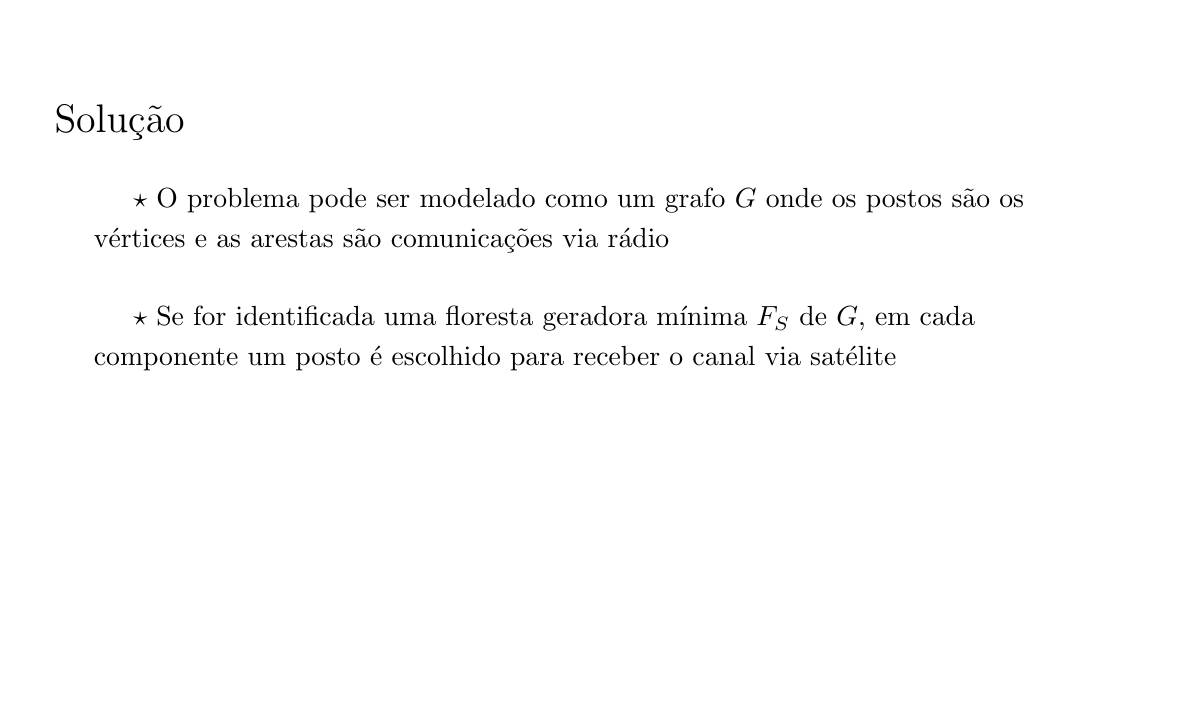
\begin{tikzpicture}
\node[draw,opacity=0] at (0, 0) {x};
\node[draw,opacity=0] at (14, 8) {x};


	\node[anchor=west] (header) at (0.0, 7.0) { \Large \bbbold{Solução} };


	\node[anchor=west] (a) at (1.0, 6.0) { $\star$ \bbtext{O problema pode ser modelado como um grafo $G$ onde os postos são os} };

	\node[anchor=west] (a1) at (0.5, 5.5) { \bbtext{vértices e as arestas são comunicações via rádio} };


	\node[anchor=west] (b) at (1.0, 4.5) { $\star$ \bbtext{Se for identificada uma floresta geradora mínima $F_S$ de $G$, em cada} };

	\node[anchor=west] (b1) at (0.5, 4.0) { \bbtext{componente um posto é escolhido para receber o canal via satélite} };


\end{tikzpicture}
\end{frame}
\begin{frame}[plain,t]
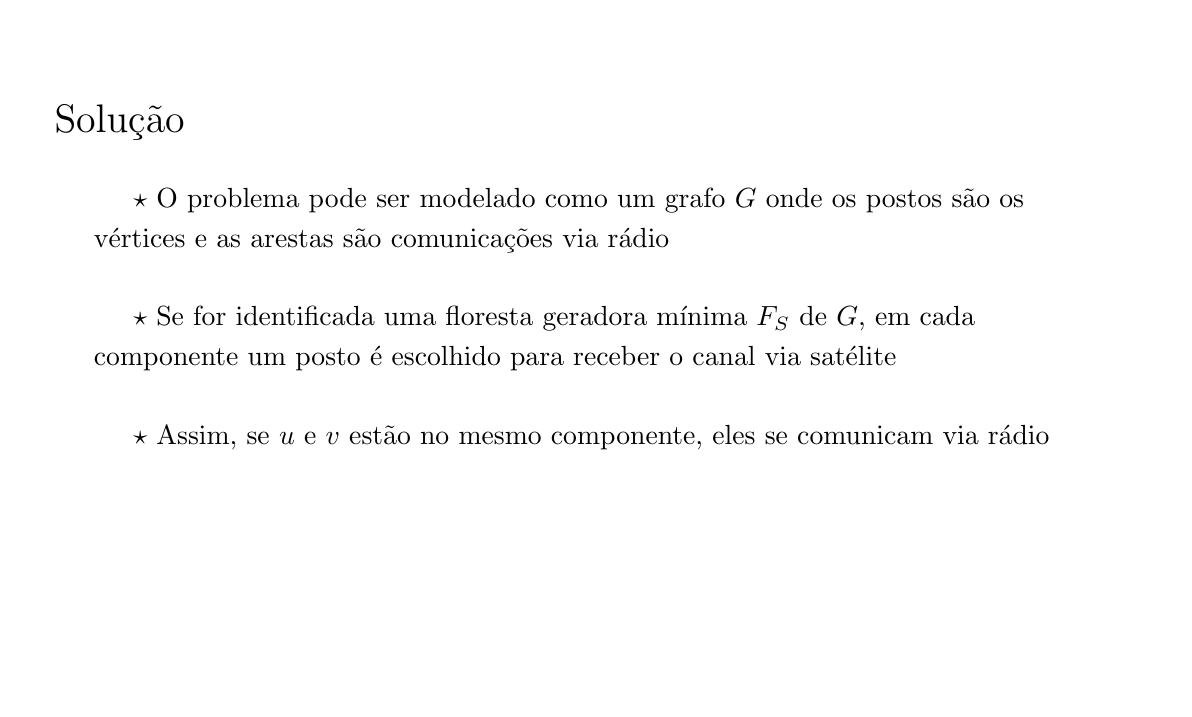
\begin{tikzpicture}
\node[draw,opacity=0] at (0, 0) {x};
\node[draw,opacity=0] at (14, 8) {x};


	\node[anchor=west] (header) at (0.0, 7.0) { \Large \bbbold{Solução} };


	\node[anchor=west] (a) at (1.0, 6.0) { $\star$ \bbtext{O problema pode ser modelado como um grafo $G$ onde os postos são os} };

	\node[anchor=west] (a1) at (0.5, 5.5) { \bbtext{vértices e as arestas são comunicações via rádio} };


	\node[anchor=west] (b) at (1.0, 4.5) { $\star$ \bbtext{Se for identificada uma floresta geradora mínima $F_S$ de $G$, em cada} };

	\node[anchor=west] (b1) at (0.5, 4.0) { \bbtext{componente um posto é escolhido para receber o canal via satélite} };



	\node[anchor=west] (c) at (1.0, 3.0) { $\star$ \bbtext{Assim, se $u$ e $v$ estão no mesmo componente, eles se comunicam via rádio} };

\end{tikzpicture}
\end{frame}
\begin{frame}[plain,t]
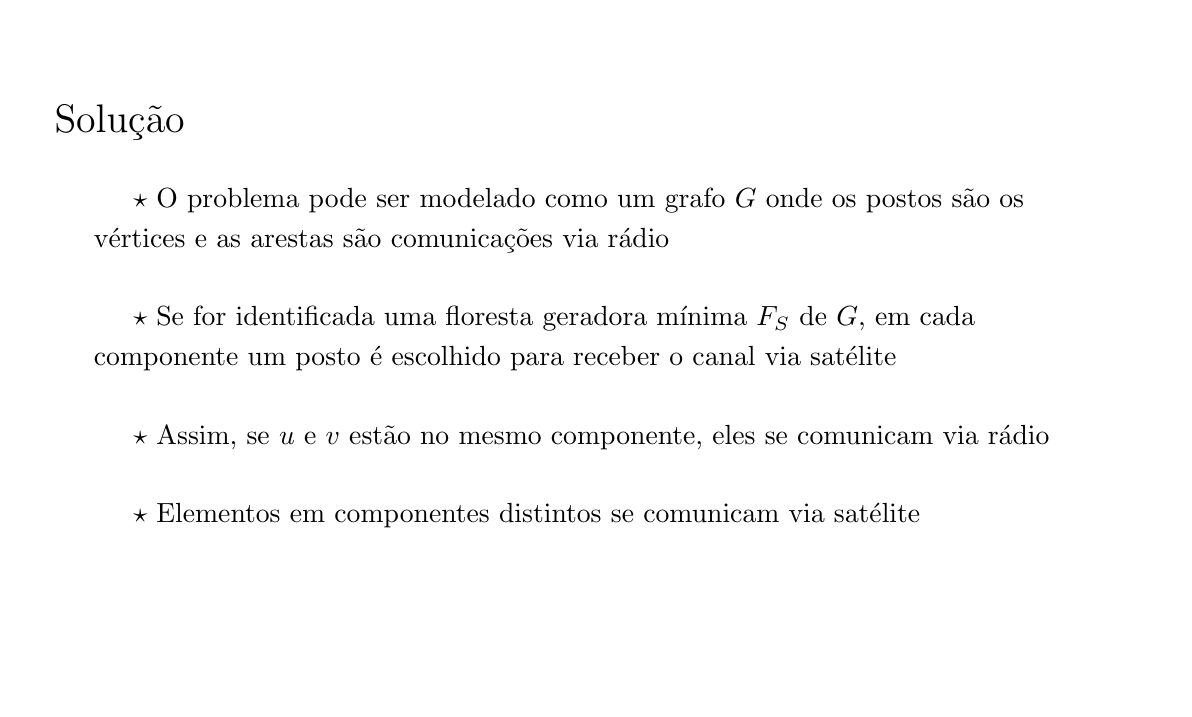
\begin{tikzpicture}
\node[draw,opacity=0] at (0, 0) {x};
\node[draw,opacity=0] at (14, 8) {x};


	\node[anchor=west] (header) at (0.0, 7.0) { \Large \bbbold{Solução} };


	\node[anchor=west] (a) at (1.0, 6.0) { $\star$ \bbtext{O problema pode ser modelado como um grafo $G$ onde os postos são os} };

	\node[anchor=west] (a1) at (0.5, 5.5) { \bbtext{vértices e as arestas são comunicações via rádio} };


	\node[anchor=west] (b) at (1.0, 4.5) { $\star$ \bbtext{Se for identificada uma floresta geradora mínima $F_S$ de $G$, em cada} };

	\node[anchor=west] (b1) at (0.5, 4.0) { \bbtext{componente um posto é escolhido para receber o canal via satélite} };



	\node[anchor=west] (c) at (1.0, 3.0) { $\star$ \bbtext{Assim, se $u$ e $v$ estão no mesmo componente, eles se comunicam via rádio} };


	\node[anchor=west] (d) at (1.0, 2.0) { $\star$ \bbtext{Elementos em componentes distintos se comunicam via satélite} };

\end{tikzpicture}
\end{frame}
\begin{frame}[plain,t]
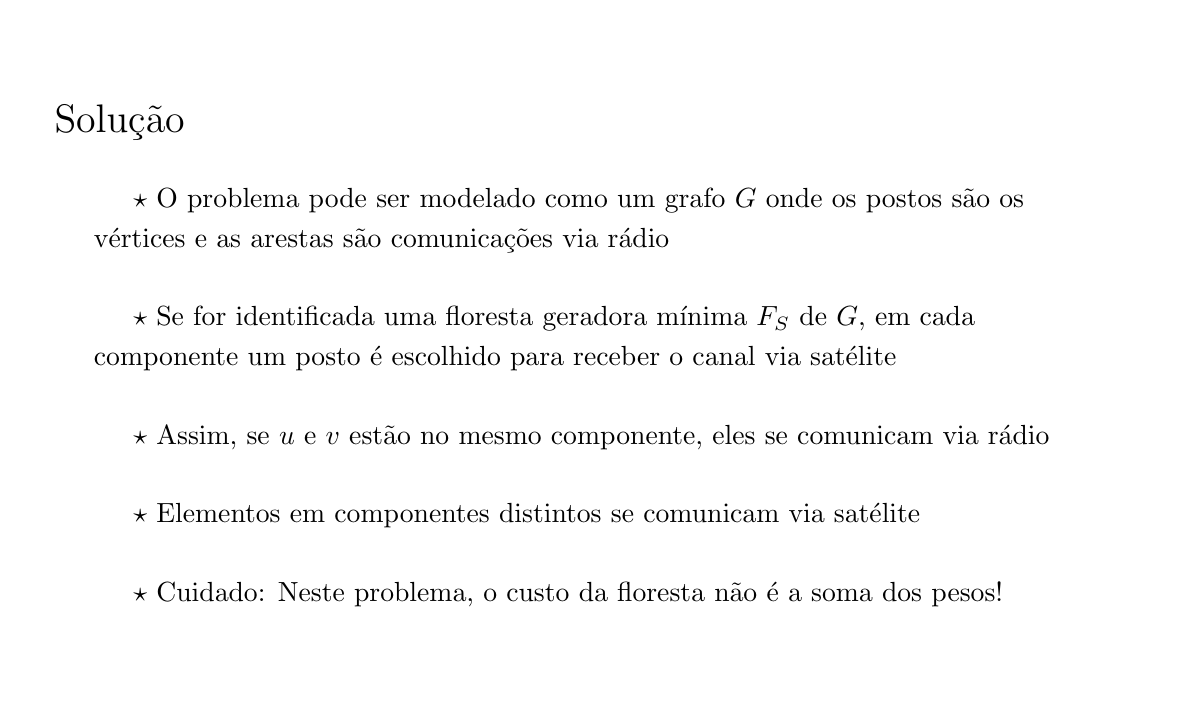
\begin{tikzpicture}
\node[draw,opacity=0] at (0, 0) {x};
\node[draw,opacity=0] at (14, 8) {x};


	\node[anchor=west] (header) at (0.0, 7.0) { \Large \bbbold{Solução} };


	\node[anchor=west] (a) at (1.0, 6.0) { $\star$ \bbtext{O problema pode ser modelado como um grafo $G$ onde os postos são os} };

	\node[anchor=west] (a1) at (0.5, 5.5) { \bbtext{vértices e as arestas são comunicações via rádio} };


	\node[anchor=west] (b) at (1.0, 4.5) { $\star$ \bbtext{Se for identificada uma floresta geradora mínima $F_S$ de $G$, em cada} };

	\node[anchor=west] (b1) at (0.5, 4.0) { \bbtext{componente um posto é escolhido para receber o canal via satélite} };



	\node[anchor=west] (c) at (1.0, 3.0) { $\star$ \bbtext{Assim, se $u$ e $v$ estão no mesmo componente, eles se comunicam via rádio} };


	\node[anchor=west] (d) at (1.0, 2.0) { $\star$ \bbtext{Elementos em componentes distintos se comunicam via satélite} };


	\node[anchor=west] (e) at (1.0, 1.0) { $\star$ \bbbold{Cuidado:} \bbtext{Neste problema, o custo da floresta não é a soma dos pesos!} };

\end{tikzpicture}
\end{frame}
\begin{frame}[plain,t]

\inputsnippet{cpp}{68}{87}{codes/10369.cpp}

\end{frame}
\begin{frame}[plain,t]

\inputsnippet{cpp}{47}{66}{codes/10369.cpp}

\end{frame}
\end{document}
